\subsection{Фотонейтринный процесс}
Еще одним процессом, в котором может реализовываться резонанс на виртуальном электроне, является фоторождение пары нейтрино-антинейтрино на электроне, $e\gamma\to e\nu\bar\nu$, называемое фотонейтринным процессом. Наряду с другими реакциями, имеющими нейтринную пару в конечном состоянии, интерес к нему связан с тем, что такие процессы могут играть важную роль в остывании нейтронных звезд, поскольку замагниченная плазма прозрачна для нейтрино при значениях параметров (плотности и температуры), которые дают все существующие модели их внутреннего строения.

Первые работы, посвященные фотонейтринному процессу, вышли в 60-ых годах прошлого века~\cite{Ritus:1961,Chiu:1961}. Нейтринная светимость, т.е. энергия, уносимая нейтринной парой из единичного объема за единицу времени, за счет него была вычислена в работах~\cite{Beaudet:1967,Dicus:1972,Munakata:1985,Shindler:1987,Itoh:1989,Itoh:1996,Skobelev:2000}. В частности, в~\cite{Itoh:1989,Itoh:1996} были получены таблицы с большим количеством данных для фотонейтринной излучательной способности и аналитические аппроксимации для них. При этом вклад реакции в процесс нейтринного остывания нейтронной звезды полагался пренебрежимо малым, как отмечают авторы обзора~\cite{Yakovlev2001}, поскольку в холодной и плотной плазме распад плазмона, $\gamma\to\nu\bar\nu$, является намного более эффективным каналом по уносу энергии за счет нейтринных пар.

На следующем этапе фотонейтринный процесс изучался с учетом влияния внешней активной среды на дисперсионные и поляризационные свойства фотона~\cite{RCh:2008,Borisov:2012,RumChMik}. Хотя в этих работах были получены уточнения к нейтринной светимости процесса, общий вывод о том, что фотонейтринный процесс является поправкой более высокого порядка к распаду плазмона, остался неизменным.

Наконец, в~\cite{Chistyakov:2014cga,qfthep2017} был рассмотрен резонанс в фотонейтринном процессе. Приведем основные выкладки этих работ.

Излучаетльная способность нейтрино, в предположении, что обратным влиянием потерь энергии и импульса на состояние 
плазмы можно пренебречь, определяется как нулевая компонента вектора энергии-импульса, передаваемого в этом 
процессе от нейтрино единице объёма внешней среды за единицу времени, и имеет 
следующий вид~\textcolor{red}{\cite{Yakovlev2001, Gvozdev:2002}}:
%                                                   
\begin{eqnarray}
\label{lumin}
Q = \frac{1}{V}\, \int \prod \limits_{i} \mathrm{d} \Gamma_i f_i \,
\prod \limits_{f} \mathrm{d} \Gamma_f (1\pm f_f) \; q'_0\,
\frac{|{\cal S}_{if}|^2}{\tau}\, ,
\end{eqnarray}
\noindent где $\dd \Gamma_i$ $(\dd \Gamma_f)$ -- число состояний начальных 
(конечных) частиц; $f_i$ $(f_f)$ -- соответствующие функции распределения, 
знак  $+$ $(-)$ отвечает конечным бозонам (фермионам); 
$q^{\, \prime}_0$ -- энергия нейтринной пары; $V = L_x L_y L_z$ -- объем плазмы, $\tau$ -- время 
взаимодействия.

${\cal S}$-матричный элемент для процесса $\gamma e\to e\nu\bar\nu$ описывается диаграммами, изображёнными на 
рис.~\ref{fig2_1} и может быть представлен в следующем виде:
%
\beq
&&{\cal S}_{\gamma e\to e\nu\bar\nu} = \frac{\ii (2\pi)^3 \delta^{(3)}_{0,y,z} (p+q-p^{\, \prime} -q^{\, \prime})}
{L_y L_z \sqrt{2^5 V^3\omega E_{\ell} E^{\, \prime}_{\ell^{\, \prime}} E_1 E_2}} {\cal M}_{\gamma e\to e\nu\bar\nu}\, ,
\eeq

\noindent Амплитуда ${\cal M}_{\gamma e\to e\nu\bar\nu}$ может быть получена 
из формулы~(\ref{eq:M12}) Главы 1 с помощью подстановок
$\Gamma_{k'} = \gamma_\alpha (C_V+C_A \gamma_5)$, 
$j^{\,\prime}_{k'} = J_\alpha$, $g_{k'} = \frac{G_F}{\sqrt{2}}$,
$\Gamma_{k} = \gamma_\beta$, $j_{k} = \varepsilon_\beta$, 
$g_{k} = e$ и имеет следующий вид:

%
\beq
&&{\cal M}_{\gamma e\to e\nu\bar\nu} = \frac{\ii e G_F}{\sqrt{2}} \sum\limits_{n=0}^{\infty} \sum\limits_{s^{\,\prime\prime} = \pm 1}
\int \dd X_1 \dd Y_1 \eee^{-\ii X_1 q_x + \ii Y_1 q_x^{\,\prime}} \times
\\
\nonumber
&&\times
\frac{\phi_{p^{\,\prime}, \ell^{\,\prime}}^{s^{\,\prime}} (Y_1) \gamma_{\alpha} J_{\alpha} (C_V+C_A \gamma_5) 
\phi_{p+q, n}^{s^{\,\prime\prime}} (Y_1) \phi_{p+q, n}^{s^{\,\prime\prime}} (X_1) \gamma_{\beta} \varepsilon_{\beta} (q) 
\phi_{p, \ell}^{s} (X_1)}{(p+q)_{\mprl}^2-M_n^2+\ii \Im_{\Sigma}^{s^{\,\prime\prime}} (p+q)} 
+
\\
\nonumber
&&+
\frac{\ii e G_F}{\sqrt{2}} \sum\limits_{n=0}^{\infty} \sum\limits_{s^{\,\prime\prime} = \pm 1}
\int \dd X_1 \dd Y_1 \eee^{\ii X_1 q^{\,\prime}_x - \ii Y_1 q_x}
\times
\\
\nonumber
&&\times
\frac{\phi_{p^{\,\prime}, \ell^{\,\prime}}^{s^{\,\prime}} (Y_1) 
\gamma_{\beta} \varepsilon_{\beta} (q) 
\phi_{p-q^{\,\prime}, n}^{s^{\,\prime\prime}} (Y_1) \phi_{p-q^{\,\prime}, n}^{s^{\,\prime\prime}} (X_1) 
\gamma_{\alpha} J_{\alpha} (C_V+C_A \gamma_5) 
\phi_{p, \ell}^{s} (X_1)}{(p-q^{\,\prime})_{\mprl}^2-M_n^2+\ii \Im_{\Sigma}^{s^{\,\prime\prime}} (p-q^{\,\prime})}\, . 
\eeq
%

\begin{figure}[h]
\centering
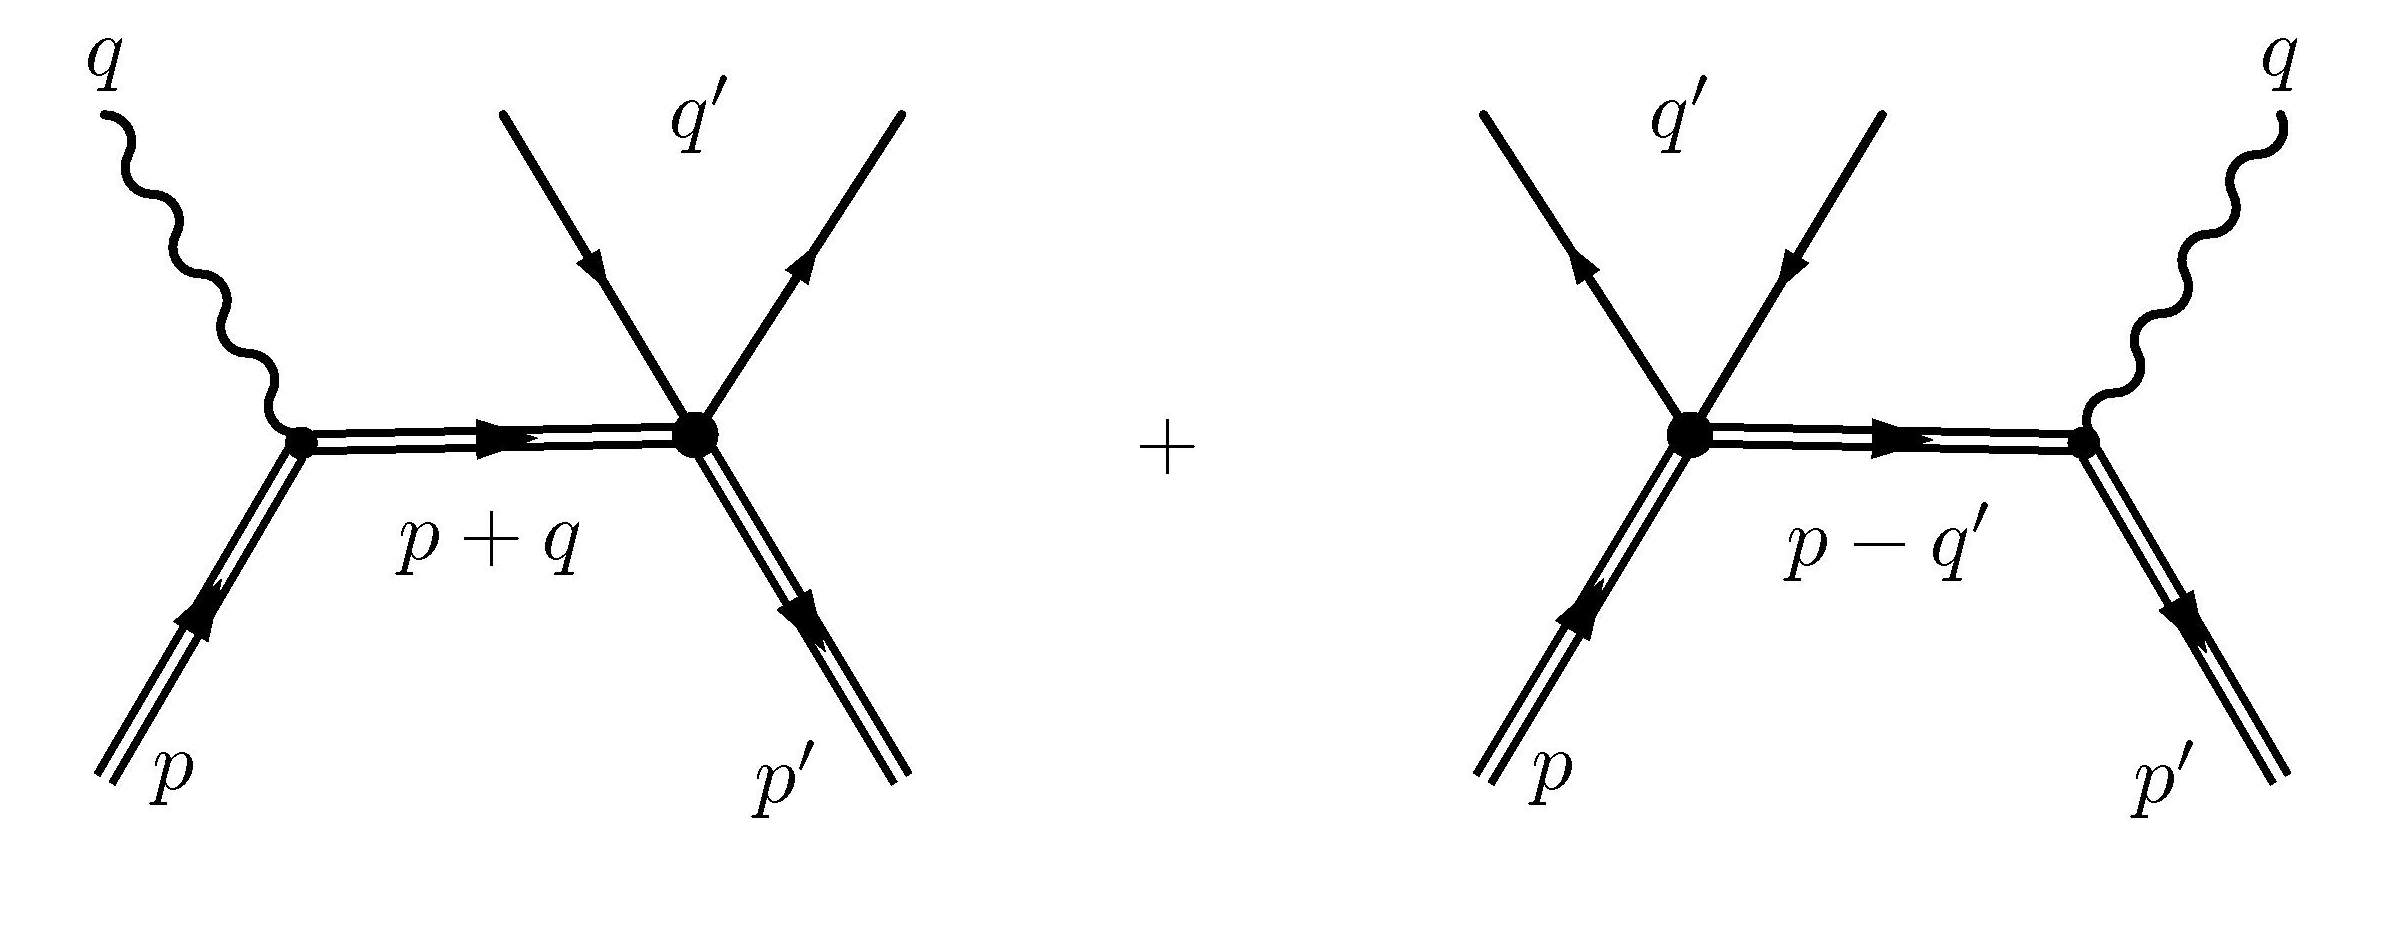
\includegraphics[width=10cm,clip]{fig2_1.jpg}
\caption{Диаграммы Фейнмана для реакции $\gamma e\to e\nu\bar\nu$. 
Двойные линии обозначают, что влияние внешнего поля на начальное и 
конечное состояние и на элеткронный пропагатор учтено точно.} 
\label{fig2_1}  
\end{figure}
%

В приближении узкого резонансного пика с учётом факторизации 
квадрата ${\cal S}$-матричного элемента~(\ref{eq:S2factor}) и выражения~(\ref{eq:Msquare})
нейтринную светимость~(\ref{lumin}) для резонансного фотонейтринного процесса можно представить в виде:
%
\beq
\label{Qres}
&&Q_{\gamma e \to e\nu \bar \nu} = \frac{1}{L_x} 
\sum\limits_{n=1}^{\infty} \;
\sum\limits_{\ell,\ell^{\,\prime}=0}^{n-1} \sum\limits_{s,s^{\,\prime},s^{\,\prime\prime}=\pm 1}
\int \frac{\dd^3 k}{(2\pi)^3 2\omega} f_{\gamma} (\omega) \frac{\dd p_y \dd p_z}{(2\pi)^2 2 E_{\ell}} 
\times
\\
\nonumber
&&\times
f_e (E_{\ell}) 
\frac{\dd p^{\,\prime}_y \dd p^{\,\prime}_z}{(2\pi)^2 2 E^{\,\prime}_{\ell^{\,\prime}}} [1-f_e (E^{\,\prime}_{\ell^{\,\prime}})]
\frac{\dd p^{\,\prime\prime}_y \dd p^{\,\prime\prime}}{(2\pi)^2 (2 E^{\,\prime\prime}_n)^2 \Gamma_n^{s''}}
\frac{\dd^3 p_1}{(2\pi)^3 2E_1} \frac{\dd^3 p_2}{(2\pi)^3 2E_2} q_0^{\,\prime}
\times
\\
\nonumber
&&\times
(2\pi)^6 \delta^{(3)}_{0,y,z} (p+q-p^{\,\prime\prime}) \delta^{(3)}_{0,y,z} (p^{\,\prime\prime} -p^{\,\prime}-q^{\,\prime})
|{\cal M}_{e_{\ell}\gamma\to e_n}|^2 |{\cal M}_{e_n \to e_{\ell'} \nu \bar \nu}|^2\, .
\eeq 

Полная ширина изменения состояния электрона может быть выражена через 
ширину рождения~\cite{Weldon:1983}:
%
\begin{eqnarray}
\label{Gns}
\Gamma_n^{s^{\,\prime\prime}} = \Gamma^{(abs)\, s^{\,\prime\prime}}_n + \Gamma^{(cr) \, s^{\,\prime\prime}}_n \simeq 
 \Gamma^{(cr) \, s^{\,\prime\prime}}_{e_n \to e_{\ell'} \gamma} 
\left [1+ \eee^{(E^{\, \prime \prime}_n - \mu)/T} \right ]
\end{eqnarray}
%
\begin{eqnarray}
\label{Gcr}
&&\Gamma_n^{(cr) \, s^{\,\prime\prime}} = \sum\limits_{\ell=0}^{n-1} \sum\limits_{s^{\,\prime\prime}=\pm 1}
\frac{1}{2E^{\,\prime\prime}_n}\int\frac{d^3 k}{(2\pi)^3 2\omega} f_{\gamma} (\omega) \times
\\
\nonumber
&&\times \frac{\dd p_y \dd p_z}{2 E_{\ell}} f_e (E_{\ell}) (2\pi)^3 \delta^{(3)}_{0,y,z} (p+q-p^{\,\prime\prime}) 
|{\cal M}_{e_{\ell}\gamma\to e_n}|^2\, ,
\end{eqnarray}
%

Подставляя~(\ref{Gns}) и (\ref{Gcr}) в формулу~(\ref{Qres}) и выполняя несложные преобразования, 
получаем следующее выражение для резонансной нейтринной светимости за счёт процесса  $e\gamma\to e\nu\bar\nu$:
%
\beq
\label{eq:Qres}
Q_{\gamma e \to e \nu \bar \nu} = \sum\limits_{n=1}^{\infty}
\sum\limits_{\ell'=0}^{n-1}  
Q_{e_n \to e_{\ell'} \nu \bar \nu}  \, ,
\eeq
\noindent где
\beq
\nonumber
&&Q_{e_n \to e_{\ell'} \nu \bar \nu} =  \frac{1}{L_x}\; \int 
\frac{\dd p_y^{\, \prime \prime} \dd p_z^{\, \prime \prime}}{(2\pi)^2 \, 
2 E_n^{\, \prime \prime}} \, f_{e} (E_n^{\, \prime \prime}) \,  
\frac{\dd p_y^{\, \prime} \dd p_z^{\, \prime}}{(2\pi)^2 \, 2 E^{\, \prime}_{\ell'} } \,
\left [1-f_{e}(E^{\, \prime}_{\ell'}) \right ] \times 
\\
\label{eq:Qnusynh}
&&\times  
\frac{\dd^3 p_1}{(2\pi)^3 \, 2 E_1} \,
\frac{\dd^3 p_2}{(2\pi)^3 \, 2 E_2} \,  
q^{\, \prime}_0\,
(2 \pi)^3  \, \delta^{(3)}_{0,y,z} (p'' - p^{\, \prime} - q^{\, \prime}) 
|{\cal M}_{e_n \to e_{\ell'} \nu \bar \nu}|^2 
\eeq
%                                                  
\noindent -- это нейтринная светимость за счёт процесса $e_n\to e_{\ell'} 
\nu\bar\nu$~\cite{Yakovlev2001}.
Квадрат амплитуды $e_n \to e_{\ell'} \nu \bar \nu$ может быть получен с помощью выражений~(\ref{V--}-\ref{A++}) Главы 1
и представлен в следующем виде:
%
\beq
\label{eq:amp_syn}
&&|{\cal M}_{e_n \to e_{\ell'} \nu \bar \nu}|^2  = \frac{16}{3} G^2_F \left (\overline{C_V^2} + \overline{C_A^2} \right ) 
\Big \{ \left [2 q^{\, \prime \,2} (\beta (n+\ell^{\, \prime}) + m^2) + m^2 q_{\mprp}^{\, \prime \,2} \right ] \times
\\[3mm]
\nonumber
&& \times \left ({\cal I}^{\, \prime \,2}_{n-1, \ell^{\, \prime}} + {\cal I}^{\, \prime \,2}_{n, \ell^{\, \prime}-1} - 
{\cal I}^{\, \prime\, 2}_{n, \ell^{\, \prime}} - {\cal I}^{\, \prime\, 2}_{n-1, \ell^{\, \prime}-1} \right ) -
q^{\, \prime \,4} \left ({\cal I}^{\, \prime \,2}_{n-1, \ell^{\, \prime}} + {\cal I}^{\, \prime \,2}_{n, \ell^{\, \prime}-1} \right ) + 
\\[3mm]
\nonumber
&& + m^2 q^{\, \prime \,2} \left ({\cal I}^{\, \prime \,2}_{n, \ell^{\, \prime}} - {\cal I}^{\, \prime \,2}_{n-1, \ell^{\, \prime}-1} \right ) \Big \} - 
G^2_F \left (\overline{C_V^2} - \overline{C_A^2} \right ) m^2 \Big \{ (2 q_{\mprl}^{\, \prime \,2} - q_{\mprp}^{\, \prime \,2})
\times
\\[3mm]
\nonumber
&& \times 
\left ({\cal I}^{\, \prime \,2}_{n-1, \ell^{\, \prime}} + {\cal I}^{\, \prime \,2}_{n, \ell^{\, \prime}-1} - 
{\cal I}^{\, \prime \,2}_{n, \ell^{\, \prime}} - {\cal I}^{\, \prime\, 2}_{n-1, \ell^{\, \prime}-1} \right )  + 
3 q^{\, \prime \,2} \left ({\cal I}^{\, \prime \,2}_{n-1, \ell^{\, \prime}} + {\cal I}^{\, \prime \,2}_{n, \ell^{\, \prime}-1} \right ) \Big \} \, .
\eeq
%
Постоянные $\overline{C_V^2}=0.93$ и $\overline{C_A^2}=0.75$ -- это результат суммирования всех каналов рождения нейтрино типов $\nu_e, \nu_\mu, \nu_\tau$.

Полученная светимость~(\ref{eq:Qnusynh}) совпадает вплоть до обозначений с 
результатами работы~\cite{Yakovlev2001}.

На рис.~\ref{QsyncQphn} представлена зависимость светимости фотонейтринного процесса от $\rho_6 = \rho /(10^6$ г/см$^3$) 
($\rho$ -- плотность плазмы) для значений параметров 
$B=50 B_e$ и $T=10^9$~К с учётом резонанса (сплошная линия) и без учёта резонанса~\cite{RumChMik} (пунктирная линия). Как видно из графика, 
вследствие влияния резонансных эффектов 
результаты для нейтринной светимости, полученные в работе~\cite{%BorKer2,
RumChMik}, 
являются заниженными при плотности $\rho\gtrsim 6\times 10^8$ г/см$^3$ и при вышеуказанных значениях магнитного поля и температуры.

\begin{figure}[h]
\centering
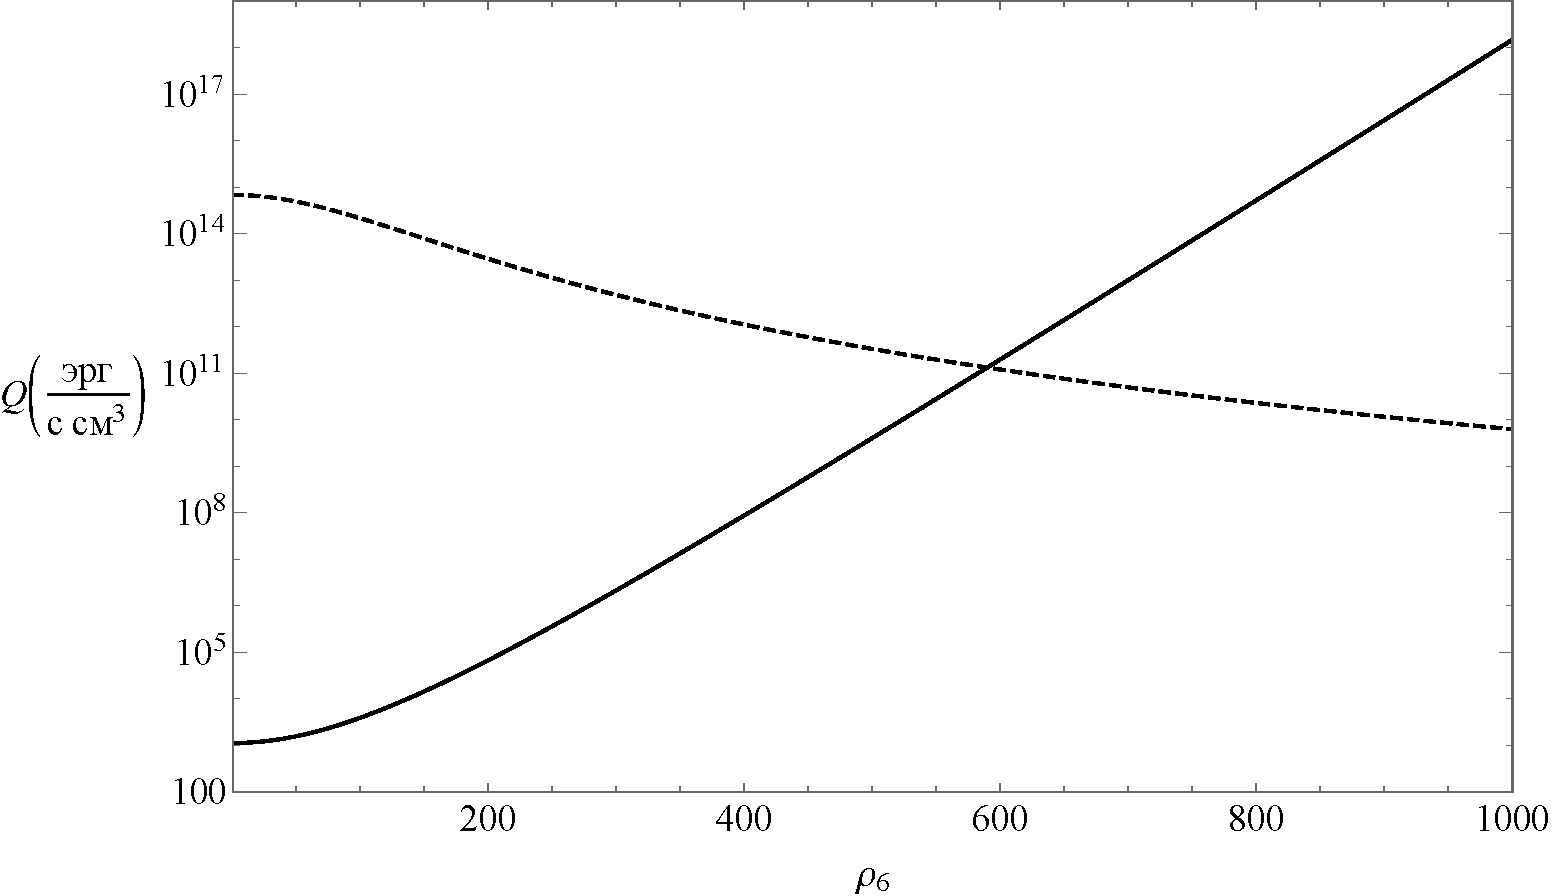
\includegraphics[width=13cm,clip]{Qsyn-Qpn 1.pdf}
\caption{Зависимость светимости фотонейтринного процесса от плотности плазмы для значений параметров 
$B=50 B_e$ и $T=10^9$~К. Сплошная линия соответствует светимости резонансного процесса, пунктирная -- без учёта резонанса.}
\label{QsyncQphn}  
\end{figure}